\documentclass[t]{beamer}
\usepackage{CJKutf8}
\usepackage{amsfonts}
    \usepackage{amsmath}
    \usepackage{amssymb}
    \usepackage{amsthm}
    \usepackage{enumerate}
    \usepackage{graphicx}
    \usepackage{layout}
    \usepackage{mathrsfs}
    \usepackage{fancyhdr}
    \usepackage{subfigure}
    \usepackage{tcolorbox}
    \usepackage{tikz-cd}
    \usepackage{color}
    \usepackage{pifont}
    \usepackage{verbatim}
    \usepackage{mathtools}
    \usepackage{float}
    \usepackage{bm}
    \usetheme{AnnArbor}
% \usetheme{Antibes}
\usecolortheme{beaver}
\usepackage{listings}

% 设置JSON样式
\lstdefinestyle{json}{
    basicstyle=\tiny\ttfamily,
    columns=fullflexible,
    showstringspaces=false,
    commentstyle=\color{gray},
    keywordstyle=\color{blue},
    stringstyle=\color{red},
    breaklines=true,
    frame=single,
    captionpos=b,
    aboveskip=10pt,
    belowskip=10pt
}

\lstset{
    language=Python, % 设置代码块语言为Python
    breaklines=true, % 自动换行
    basicstyle=\small\ttfamily, % 设置基本字体样式
    keywordstyle=\bfseries\color{blue}, % 设置关键字样式
    commentstyle=\itshape\color{gray}, % 设置注释样式
    showstringspaces=false, % 不显示字符串中的空格
    frame=single, % 设置代码块边框样式
    numbers=left, % 行号显示在左侧
    numberstyle=\tiny\color{gray}, % 设置行号样式
    stepnumber=1, % 设置行号间隔
    tabsize=4 % 设置制表符宽度
}


% 设置shell样式
\lstdefinestyle{shell}{
    language=bash,
    basicstyle=\tiny\ttfamily,
    columns=fullflexible,
    showstringspaces=false,
    commentstyle=\color{gray},
    keywordstyle=\color{blue},
    stringstyle=\color{red},
    breaklines=true,
    frame=single,
    captionpos=b,
    aboveskip=10pt,
    belowskip=10pt
}

\usepackage{subfigure}

% 添加网址的命令
\usepackage{hyperref}
% 这是一个带链接文本的示例:\href{https://www.example.com}{点击这里访问网站}
% 普通的示例:\url{https://www.example.com}
% 表格
\usepackage{booktabs}
\usepackage{multirow}

% \setbeamertemplate{navigation symbols}{}

\usepackage{textpos}

\newcommand{\dif}{\mathrm{d}}
\newtheorem{thm}{{定理}}

% some common command
\newcommand{\mm}[1]{$ #1$\newline}
% \newcommand{\tuichu}{\Rightarrow}
% \newcommand{\li}[1]{\newline#1}



\newcommand{\analysis}[2]{\forall \mathcal{E}{#1},\exists \delta {#2},s.t.}
\newcommand{\denyanalysis}[2]{\exists \mathcal{E}{#1},\forall \delta {#2},s.t.}
\newcommand{\yield}{\Rightarrow }
\newcommand{\jj}{\newline}
\newcommand{\ff}[1]{$ #1$}   % math environment + newline
\newcommand{\fgn}[1]{\begin{equation}#1\end{equation}  }
\newcommand{\fg}[1]{$$ #1$$}   % math environment + newline 
\newcommand{\pf}{$proof.$\newline}
\newcommand{\ee}{\newline\ff{\Box}\newline}
\newcommand{\fenshi}[2]{\ff{\frac{#1}{#2}}}
\newcommand{\shenlue}{\vdots\jj}
\newcommand{\abs}[1]{{\left \lvert #1 \right\rvert}}
\newcommand{\loge}[1]{In ({#1})}
\newcommand{\logical}[2]{log_{#2}^{#1}}
\newcommand{\summary}[3]{$\sum_{{#1}={#2}}^{#3}  $}
\newcommand{\denjia}[2]{{#1}\Leftrightarrow {#2}}
\newcommand{\jihe}[3]{ {#1}  = \{ {#2} \mid {#3} \} }
\newcommand{\ve}[2]{\left\langle {#1},{#2}\right \rangle}
\newcommand{\dakuohao}[2]{\begin{array}{rcl}{#1}\end{array} \} \Rightarrow{#2}}
\newcommand{\sxb}[3]{#1^{#2}_{#3}}
\newcommand{\sss}[2]{#1^{#2}}
\newcommand{\xxx}[2]{#1_{#2}}
\newcommand{\bri}[1]{\uppercase\expandafter{\romannumeral#1}}
\newcommand{\ri}[1]{\romannumeral#1} 
\newcommand{\polynomial}[8]{#1_{#2}#6^{#7}+#1_{#3}#6^{#8}+...+#1_{#4}#6+#1_{#5} }
\newcommand{\newd}[4]{f[{#1}_{#2},{#4},{#1}_{#3}]}
\newcommand{\lb}[2]{\begin{align*}\begin{split}{#1}\{ {#2}\end{split}\end{align*}}
\newcommand{\tab}[1]{\begin{array}{ll} {#1}\end{array}}


% 向量乘积
\newcommand{\avg}[1]{\left\langle #1 \right\rangle}
% 偏微分方程
\newcommand{\difFrac}[2]{\frac{\dif #1}{\dif #2}}
\newcommand{\pdfrac}[2]{\frac{\partial{#1}}{\partial{#2}}}
% 不同章节
\newcommand{\one}[1]{\section{#1}}
\newcommand{\two}[1]{\subsection{#1}}
\newcommand{\three}[1]{\subsubsection{#1}}
\newcommand{\aone}[1]{\section*{#1}}
\newcommand{\atwo}[1]{\subsection*{#1}}
\newcommand{\athree}[1]{\subsubsection*{#1}}
% 大括号,左右都有
\newcommand{\lbra}[1]{\left\{  {\begin{matrix} #1 \end{matrix}}\right. } 
% 样式 括号前缀 + 括号 
\newcommand{\lbras}[2]{{#1}\left\{ {  {\begin{matrix} #2 \end{matrix}}}\right. } 
\newcommand{\rbra}[1]{ \left.  {\begin{matrix} #1 \end{matrix}} \right\}  } 
% 模长
\newcommand{\distance}[1]{\parallel #1\parallel }
% 等价
\newcommand{\equ}{\Longleftrightarrow }
% 共轭
\newcommand{\cja}[1]{\overline{#1}}
% 两个矩阵,上面是 方框[] 下面是线条| 中间是 无
\newcommand{\mtx}[1]{\begin{matrix}#1\end{matrix} }
\newcommand{\bmtx}[1]{\begin{bmatrix}#1\end{bmatrix} }
\newcommand{\vmtx}[1]{\begin{vmatrix}#1\end{vmatrix} }
% \newcommand{\table}[1]{\begin{array}[lr]{ccc} #1 \end{array}}

%输入普通字符
\newcommand{\ww}[1]{\text{#1}}

% 所有内容 直接头文件搞定
\newcommand{\everything}[1]{\begin{document}\begin{CJK*}{UTF8}{gkai}#1\end{CJK*}\end{document}}


% 存放代码(失败了)
\newcommand{\cccode}[1]{\begin{lstlisting}#1\end{lstlisting}}

% 改变特定行序列
\newcommand{\ttt}{\subsection{}}

% 嵌套序号
\newcommand{\eee}[1]{\begin{enumerate}#1\end{enumerate}}


% 模板里面的一些宏
\newcommand{\pdfFrac}[2]{\frac{\partial #1}{\partial #2}}
\newcommand{\OFL}{\mathrm{OFL}}
\newcommand{\UFL}{\mathrm{UFL}}
\newcommand{\fl}{\mathrm{fl}}
\newcommand{\op}{\odot}
\newcommand{\Eabs}{E_{\mathrm{abs}}}
\newcommand{\Erel}{E_{\mathrm{rel}}}
% 变化颜色
\newcommand{\red}{\textcolor{red}}
\newcommand{\blue}{\textcolor{blue}}
% 注释代码
% \newcommand{\undef}[1]{\iffalse #1 \fi}

% 流程图需要用到的宏包
\usepackage{palatino}
\usepackage{tikz}
\usetikzlibrary{shapes.geometric, arrows}
\tikzstyle{startstop} = [rectangle, rounded corners, minimum width = 2cm, minimum height=1cm,text centered, draw = black, fill = red!40]
\tikzstyle{io} = [trapezium, trapezium left angle=70, trapezium right angle=110, minimum width=2cm, minimum height=1cm, text centered, draw=black, fill = blue!40]
\tikzstyle{process} = [rectangle, minimum width=3cm, minimum height=1cm, text centered, draw=black, fill = yellow!50]
\tikzstyle{decision} = [diamond, aspect = 3, text centered, draw=black, fill = green!30]
% 箭头形式
\tikzstyle{arrow} = [->,>=stealth]
% 4个非常重要 的新命令
\newcommand{\start}[2]{    \node (start) [startstop]{#1};\node (in1) [io, below of = start]{#2};\lin{start}{in1}{}}
\newcommand{\stopp}[3]{\node (out1) [io, below of= #1]{#2};\node (stop) [startstop, below of=out1]{#3};\lin{out1}{stop}{} }
\newcommand{\pro}[6]{    \node (#3) [process, #2 of=#1,xshift=#4 cm]{#5};}
\newpage
\newcommand{\lin}[3]{\draw [arrow] (#1) --node [above] {#3} (#2);}


\begin{document}
\begin{CJK*}{UTF8}{gkai}
% 一般第一页显示PPT标题以及作者信息

% \BackgroundPic{./Screenshot from 2022-04-20 16-31-08.png}

% 增加学校 前面
\addtobeamertemplate{title page}{}{
	\begin{tikzpicture}[remember picture,overlay]
		% \node[yshift=85pt,xshift=50pt]{\includegraphics[height=2cm]{Screenshot from 2022-04-20 16-51-21.png}};
\end{tikzpicture}
}
	% \title{时间序列数据集}
	\title{组会汇报}
	\subtitle {} %不需要
	\author{
		陈钶杰\, \\
		专业:计算数学\,
	} % 显示作者
	% \institute {学院:数学科学学院} % 设置学院机构	
	\date{\today}  % 显示日期
\titlepage

    % 设置目录
\begin{frame}{目录}
\frametitle{目录}	
\tableofcontents  % 显示目录
\end{frame}

% \section{相关文献阅读-MLC模型}

\section{模型构建}

\begin{frame}
    \frametitle{3进制的多位数加法}
    主要任务:
    \eee{
        \item 数字对齐
        \item 数字计算
        \item 数字进位
        \item 模型目标:\\
        input:['2','2','+','1']\\
        output:['1','1','0']
    
    }    
\end{frame}

\subsection{数字对齐}
\begin{frame}
    \frametitle{数字对齐}
    \begin{itemize}{
        \item 通过学习对齐规则,对每次输入的数据进行对齐
        \item 目标\\
        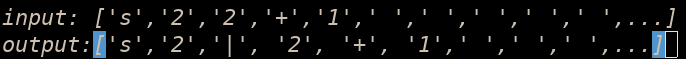
\includegraphics[scale=0.3]{png/compute1.png}
        \item  \ \\
        \eee{
            \item 三进制的对齐规则:
            \item 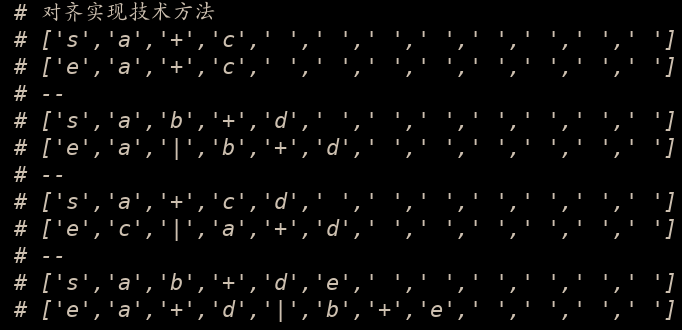
\includegraphics[scale=0.3]{png/regular-aligon.png}
        }
        }    
    \end{itemize}
\end{frame}

\subsection{数字计算}
\begin{frame}
    \frametitle{思路}
    \eee{
        \item 目前还未有比较好的方法,如果使用for循环是否会有不妥
        \item  目标:\\
        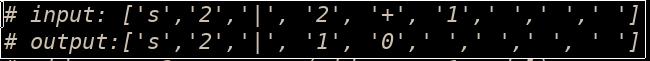
\includegraphics[scale=0.3]{png/compute.png}
    }
\end{frame}

\subsection{数字进位}
\begin{frame}
    \frametitle{数字进位}
    \begin{itemize}
        \item 通过学习进位规则,对每次输入的数据进行进位
        \item 目标\\
        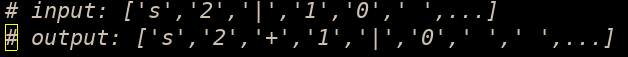
\includegraphics[scale=0.3]{png/compute2.png}
        \item \ \\
        \eee{
            \item 三进制的进位规则:
            \item 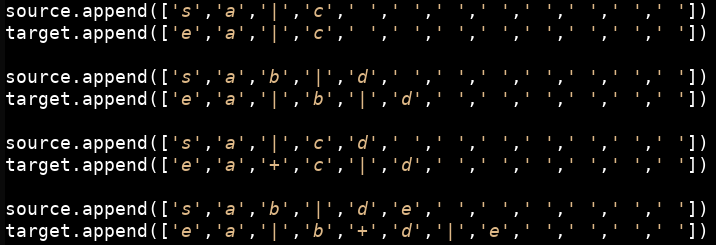
\includegraphics[scale=0.3]{png/regular-jin.png}
        }
    \end{itemize}    
\end{frame}

\begin{frame}
    \frametitle{模型信息}
    \begin{itemize}
        \item 数据组成:\\
        \eee{
        \item 基本3以内的加法
        \item 进位规则
        \item 对齐规则
        }
        \item 模型:transformer
    \end{itemize}
\end{frame}

\begin{frame}
    \frametitle{下一步计划}
    \eee{
        \item 实现中间步骤的计算
        % \item 进行模型相关修改
        }
\end{frame}

% \begin{frame}
%     \frametitle{MathGPT构建模型策略}
%     \begin{itemize}
%         \item MathGLM的模型构建策略:\\
%         \eee{
%             \item 我们采用分步策略构建 算术数据集,作为MathGLM预训练的基础。该数据集旨在涵盖广泛的算术运算,从简单的一元运算到更复杂的九元运算。通过采用这种循序渐进的策略,MathGLM 学会了处理简单和复杂的算术表达式,这使得它能够准确地执行计算,即使是涉及大于8位的数字乘法以及小数和分数的乘法运算。
%             \item 算术任务大致可以分为基本算术运算和复杂混合运算。基本算术运算包含基本的数学任务,这些任务围绕着进行涉及两个数字的简单计算。另一方面,算术任务还涵盖复杂的混合运算领域,这需要管理不同算术运算和数字格式的组合的技能。
%             \item 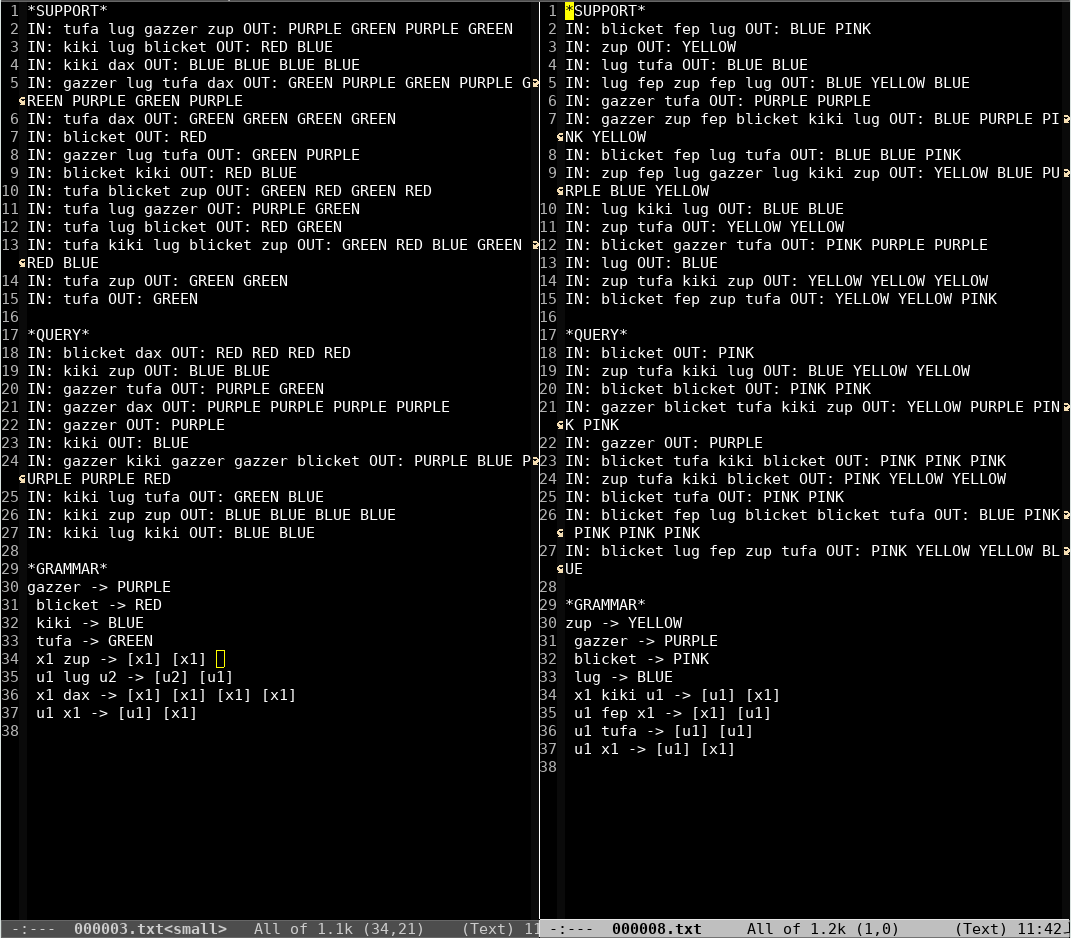
\includegraphics[scale=0.3]{png/regular.png}            
%         }
%     \end{itemize}

% \end{frame}

% \begin{frame}
%     \frametitle{}
%     \begin{itemize}
%         \item 为了增强 MathGLM 的算术能力,我们采用基于Transformer的仅解码器架构,并使用\red{自回归}目标在我们生成的算术数据集上从头开始训练它。
%         \item 它还包含多种数字格式,例如整数、小数、百分比、分数和负数。这个综合数据集以各种规模创建,范围从 100 万到 5000 万条记录。在每个数据集中,单个算术表达式由 2 到 10 个运算步骤组成,涵盖一系列数学运算,例如加法 (+)、减法 (-)、乘法 (×)、除法 (/) 和求幂(\^)。
%         \item 为了符合人类的计算习惯,在算术数据集的构建中采用了分步策略。该策略不是直接计算每个复杂算术表达式的最终答案,而是将复杂表达式分解为一系列更简单的步骤,逐步生成答案。这种策略反映了人类在解决复杂算术任务时通常遵循的过程。通过在这样的数据集上进行训练,MathGLM 获得了出色的算术性能,因为它从详细的计算过程中学习了底层的计算规则。
%         % 图 3 提供了从算术数据集中提取的一些训练示例,说明了算术任务的多样性以及数据集中包含的分步策略。
%     \end{itemize}
    


% \end{frame}
% \begin{frame}
%     \frametitle{模型相关参数}
%     \begin{itemize}
%         \item 我们的训练工作包括 4 种不同类型的模型,每种模型都有不同的参数大小。最大的模型被赋予2B参数,容量最强。接下来,我们训练具有 500M 参数的第二个模型,具有 100M 参数的第三个模型和具有 10M 参数的最小模型。值得注意的是,尽管参数大小存在差异,但所有模型均使用由5000万条训练记录组成的相同数据集规模进行训练。MathGLM 的训练过程是使用包含5位数字范围内的数字的算术数据集启动的。\\
%         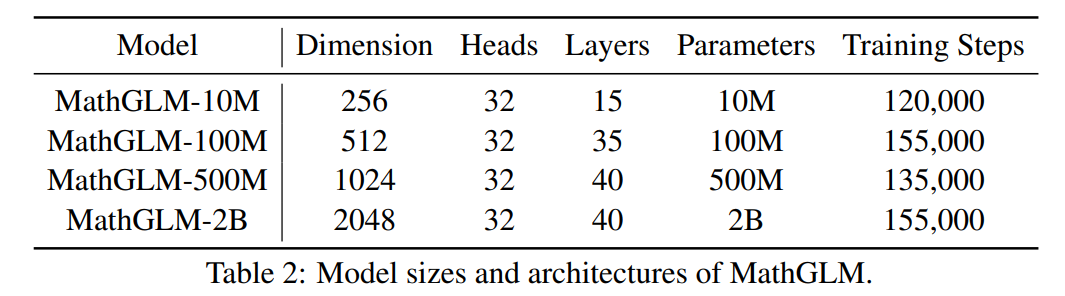
\includegraphics[scale=0.3]{png/math-glm-model.png}        
%     \end{itemize}
% \end{frame}


% \begin{frame}
%     \frametitle{MathGLM模型的训练集}
%     % 这些是提供了从算术数据集中提取的一些训练示例,说明了算术任务的多样性以及数据集中包含的分步策略。
    
%     \begin{itemize}
%         \item MathGLM 的训练过程是使用包含 5 位数字范围内的数字的算术数据集启动的。在这个初始阶段之后,MathGLM 实现了稳定的训练收敛并在测试数据集上表现出了令人满意的性能,我们引入课程学习来增强其能力。具体来说,我们使用包含 50,000 条记录的新数据集来扩充训练数据,其中包含 5 到 12 位数字的数字。\\
%         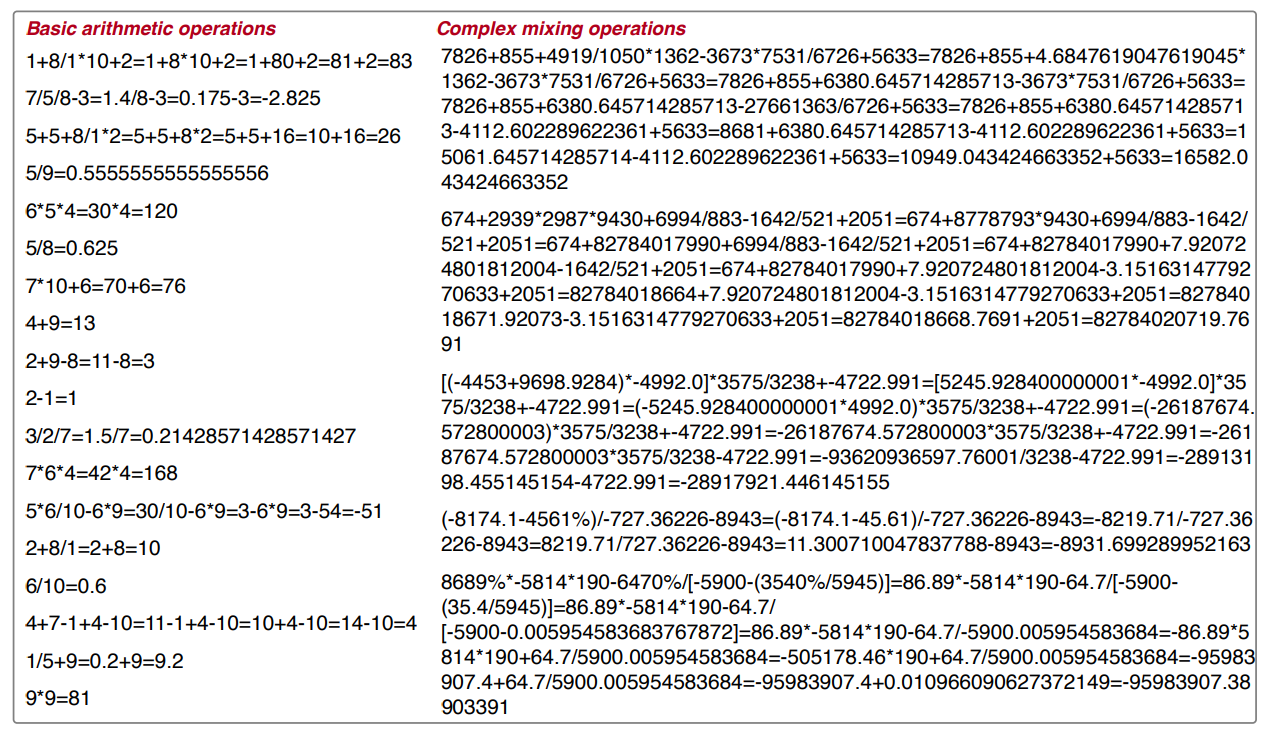
\includegraphics[scale=0.15]{png/math-glm-train.png}\\
%     \end{itemize}

% \end{frame}

% \begin{frame}
%     \frametitle{}
%     \begin{itemize}
%         \item 模型特点
%         \eee{
%             \item 这种训练策略使 MathGLM 能够首先解决更简单的示例,然后逐步应对更复杂的挑战。更重要的是,这种方法使MathGLM能够通过从相对较小的示例中学习来提高其能力,强调MathGLM处理日益复杂的任务或数据模式的效率。
%             \item 为了获得更好的性能,我们对 MathGLM 采用了两种训练策略。第一个是在单独的数学数据集上微调 GLM 主干模型。此过程使 MathGLM 能够通过学习数学数据集的独特特征来专门理解和解决数学应用问题。然而,这种策略损害了 MathGLM 的通用能力。为了规避这一限制,第二种策略是继续在结合了数学和文本内容的混合数据集上训练 GLM 主干模型。这有助于平衡数学应用题的专业化与保留 MathGLM 的通用能力。
%         }
%         \item 模型评估指标:\\
%         \eee{
%             \item 准确性通常是通过比较 MathGLM 的输出和真实答案来衡量的。在我们的实验中,我们遵守标准舍入规则,限制生成的答案精确到小数点后两位。当正确舍入的答案与 MathGLM 生成的答案一致时,我们将此结果分类为正确答案。
%             \item 相对误差是用于评估 MathGLM 有效性的另一个重要指标,它量化了 MathGLM 生成的输出与正确答案之间的差异。相对误差 (RE) 使用以下公式进行量化:
%                 \fg{
%                     RE = \abs{\frac{\hat{y} - y }{y}}
%                 }
%                 出于评估目的,我们使用 1\% 的相对误差阈值。该阈值用作确定 MathGLM 生成的答案的可接受性的标准,其中落在该阈值范围内的任何相对误差都被视为准确的结果。
%         }                
%     \end{itemize}
% \end{frame}
% \begin{frame}
%     \frametitle{}
%     \eee{
%         \item 现存的一些问题:\\
%         \eee{
%             \item 模型可能会对“大于”或“小于”等不明确的短语进行不同的解释,从而导致解决方案不准确。此外,MathGLM-GLM-10B 往往难以解决涉及复杂数学运算的问题。因此,它可能会提供部分正确的算术解决方案,但无法得出最终的正确答案。
            
%         }   
%         \item 模型结果:\\
%         \eee{
%             \item 在本文中,我们的主要重点是评估法学硕士的数学推理能力,包括算术运算和数学应用题。对于算术任务,我们结合分步解决方案和课程学习,从头开始训练基于 Transformer 的语言模型。通过对大量数据的全面训练,我们建立了一个拥有 20 亿个参数的语言模型,可以在多位数算术任务中实现出色的精度,远远超过 GPT-4 的结果。这一发现令人信服地挑战了普遍的认知,即法学硕士在执行精确算术运算时面临限制,尤其是在不依赖外部计算辅助的情况下处理多位数、小数和分数时。当转向数学应用题时,我们重建了一个富含多步算术运算的数据集。在对源自 GLM-10B 的改进数据集上的 MathGLM 进行微调后,它在 5,000 个样本的中国数学问题测试集上实现了与 GPT-4 类似的性能,展示了其强大的实力。
%         }     
%     }
% \end{frame}

% \begin{frame}
%     \frametitle{模型结果:}
%     \begin{itemize}
%         \item   \ \\
%         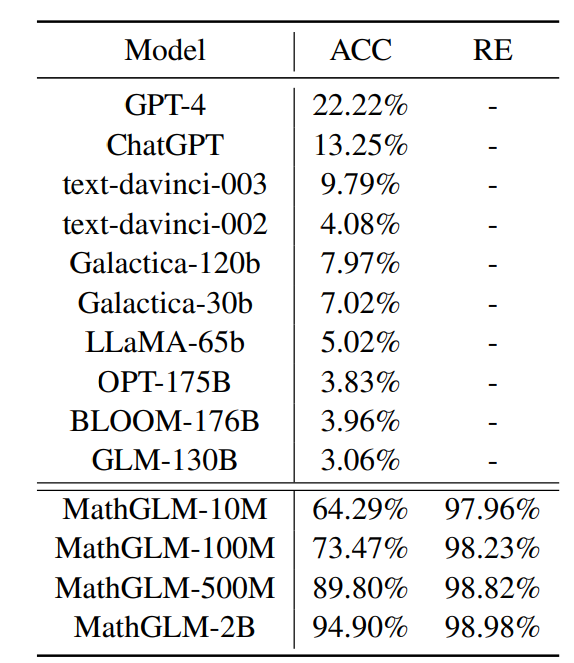
\includegraphics[scale=0.3]{png/result.png}
%     \end{itemize}
% \end{frame}


% \begin{frame}
%     \frametitle{一些可以看的参考文献}
%     \eee{
%         \item 这篇文章引入了一种新颖的架构,使模型能够捕获长期依赖关系,这有利于解决多步数值问题。[28]
%         % Dai, Z., et al., “Transformer-XL: Attentive Language Models beyond a FixedLength Context,” Proceedings of the 57th Annual Meeting of the Association for
%         % Computational Linguistics (ACL 2019), pp. 2978-2988, 2019
%         \item 这篇文章是一个用于数学问答的数据集和系统,它将自然语言理解与代数推理相结合来解决数学问题。[31]
%         % Wang, Y., et al., “MathQA: Towards Interpretable Math Word Problem Solving
%         % with Operation-Based Formalisms,” Proceedings of the 2019 Conference of the
%         % North American Chapter of the Association for Computational Linguistics: Human
%         % Language Technologies (NAACL-HLT 2019), pp. 2357-2367, 2019.
%         \item 将llm与数值优化技术相结合来解决数学规划问题,证明了比单独llm的性能有所提高.[32]
%         %  Akchurin, E., et al., “Solving Mathematical Programming Problems in Natural
%         % Language with Transformers,” arXiv preprint arXiv:2109.08601, 2021.
%         \item 工作侧重于整合外部知识源,例如知识图或数据库,以提高法学硕士在需要特定领域专业知识的任务上的表现[29,30]
%         \item 其他的代码模型[13][35]
%     }
% \end{frame}

% \begin{frame}
%     \frametitle{展望}
%     \eee{
%         \item 一个潜在的研究领域是将代码模型与外部数据源和 API 集成以对信息量进行计算。例如,通过将代码模型连接到数据库,ComputeGPT 可以帮助用户计算两个国家之间的人口差异,或分析历史数据进行预测。这将进一步增强语言模型解决数值问题的能力,并将其适用性扩展到更广泛的任务。
%         \item 开发技术来提高 ComputeGPT 生成的代码的可解释性和可解释性
%         \item 这项工作有助于越来越多的关于利用外部资源增强语言模型的研究,并为开发更高效、更强大的问题解决工具开辟了新途径。
%     }

% \end{frame}

% \begin{frame}
    % \frametitle{这周主要做的事情}
    % \eee{
        % \item 修改了训练数据集的大小,测试模型的泛化能力对于训练数据量的要求,探索模型在少量数据的情况下模型的泛化能力.可以说明一下具体修改数据量的过程
        % \item 看看老师要我看的那篇文章,快速阅读一下吧,看看有没有啥
        % \item 训练MLC模型,使其具有数字理解能力,并对结果进行展示.
        % \eee{
            % \item 我尝试了单独的乘法,加减法,发现前者效果不佳,后者效果良好(ok)
            % \item 我尝试了所有混合情况的结果,总体来说就是需要训练足够多的次数才能跑出良好的效果,所以我要在等等,才能让他跑出比较快的效果.(在两个服务器上开始跑代码,有点慢)
            % \eee{
            %     \item 这个综合任务上单独加法减法乘法上效果都良好。
            %     \item 在特殊的任务上效果一般,还在调试。
            %     (设置一套完整的参数,控制support出现次数得限制住,然后再使得最终结果尽可能的好,配置好对应参数)
            %     先设置一下对应参数吧。
            %     \item 很奇怪为啥表现一点都不好啊,我重新来理一下我的思路吧,我究竟想干嘛?
            % }
            % \item 我想做一件什么样的事情?(模型目的)
            % \eee{
            %     \item 让模型能够具有数字理解能力,比如对于模型而言知道什么1,2,...,9,知道什么是加法,知道什么是减法,知道什么是乘法?
            %     \item 如何体现模型具有数字理解能力就是让模型去做一些数字相关的问题,尝试让他把所有问题都回答出来.
            %     \item 
            %     模型的做法是这样得:\\
            %     比如我先教你一遍1+1等于几? 
            %     然后你先回答我教你的1+1 是否等与2?
            %     在然后你回答1+1+1+1+1+1等与几 6?
            %     能否回答2 + 2 等于4?
            %     最后发现这个模型在经过我教会他1+1等于2以后,他能回答出1+1+...+1= 6?
            % }

            % \item 目前在这个基本加减法和乘法效果良好,基本能达到百分百,但是对于更加复杂点的运算就不行了。想办法让他在更加复杂的运算上也能有效果?(我懂了,在我训练任务中见过的效果都是可以的,但是在训练任务中没见过的,效果是不好的,比如我在训练任务中教过他类似1 + 3 - 3怎么计算,那么对于所有的数他都是可以算出来的,不然就不会。)
            % \item 可以看看效果
            % \item 开始尝试更多更高位数的算法,看看效果会怎么样?或者写一个接口,专门针对数据的输入和输出.(等代码跑玩)
            % }
        % \item 在原有的lstm模型基础上添加了注意力机制查看是否有明显效果提升.
        % \eee{
            % \item 尝试在编码器和解码器上都添加注意力机制以后发现效果并不好,甚至不如原来的结果.我直接换别人的模板试试看吧.()
            % \item 我在我的解码器上单独设定注意力机制,看看效果是否有显著的提升吧 (ing)
            % \item 说实话我不是很理解这个过程感觉加这个注意力机制都是很麻木的,没有任何得意义啊.(我有时间加注意力机制还不如去学习一下到底什么是注意力机制,并把那些变式全部给他理解了,也当我学的八股文之一吧,反正我打算继续就这样试试看吧.至少效果不会太好的)
        % }
        
    % }
% \end{frame}

\iffalse    
\begin{frame}   
    \frametitle{文献摘要}
    作者的主要贡献:
    \eee{
        \item 我们发现,对任务多样性较低的数据进行预训练的 Transformer 的行为类似于具有先前 TPretrain 的贝叶斯估计器;它在预训练任务上表现最佳,但无法在上下文中学习新任务。然而,随着预训练任务多样性的增加,PT 偏离了这个贝叶斯估计器,在新任务上显着优于它,并且在大量但仍然有限的预训练任务中,PT 的性能与 T 上的最优估计器的性能非常接近。
        \item 我们确定了 ICL 出现的任务多样性阈值。低于此阈值,增加预训练数据集大小,同时保持任务多样性恒定,会使 PT 偏向于预训练任务分布。相反,超过这个阈值,在不增加任务多样性的情况下增加数据集大小可以提高 PT 在新的、未见过的任务上的性能。这表明 PT 的行为在每个任务的许多示例的限制下经历了急剧的算法相变,与阈值之前的 TPretrain 和阈值之后的 TPretrain 上的最佳估计器保持一致。我们还从学习动态的角度来研究这种转变。
        \item 我们的经验表明,在固定 SNR 下增加任务维度会增加任务多样性阈值。然而,PT 误差随维度的缩放比例远远优于 TPretrain 的最佳贝叶斯估计量;当任务多样性超出我们考虑的所有维度的阈值时,随着维度的增加,PT 保持接近最优,而 TPretrain 的最优估计量逐渐与 T 的最优估计量变得越来越不相似。
        \item 我们表明,增加权重衰减会显着降低任务多样性阈值,而增加层数或嵌入大小会增加任务多样性阈值。这阐明了正则化和模型容量对 ICL 出现的影响。 
        \item 图 2:ICL 在 PT 中出现,超出了预训练任务多样性的阈值。我们显示了预训练期间(顶行)和新任务(底行)期间看到的任务的所有结果。左栏将随着任务多样性的增加而预训练的 Transformer 的归一化损失与 dMMSE 和 Ridge 的归一化损失进行了比较。当预训练任务多样性较小时,PT的性能与dMMSE相匹配;它在预训练期间的任务上表现很好,但在新任务上表现不佳。随着预训练任务多样性的增加,dMMSE 和 PT 都接近 Ridge。然而,PT 接近 Ridge 的速度要快得多,在新任务上显着优于 dMMSE(左下)。在中间和右列中,我们分别将 PT 的预测与 dMMSE 和 Ridge 的预测进行比较(等式(4))。我们还通过增加批量大小,同时保持总训练步骤固定,来增加每个任务多样性级别上每个任务的序列数量。这揭示了 2 个和 2 个预训练任务之间的任务多样性阈值,在该阈值下模型的行为存在相变。低于阈值,增加数据集大小会导致 PT 的预测与 TPretrain 上的 dMMSE 更加一致(上中)。然而,超过这个阈值(由灰色阴影表示),增加数据集大小会导致 PT 在所有任务上与 Ridge 更加一致(右)。
    }
\end{frame}
\fi

% \begin{frame}
%     \frametitle{NLP相关知识}
%     \begin{itemize}
%         \item 神经网络的学习可能只是对数据集的压缩.\\
%         图像说明:\\
%         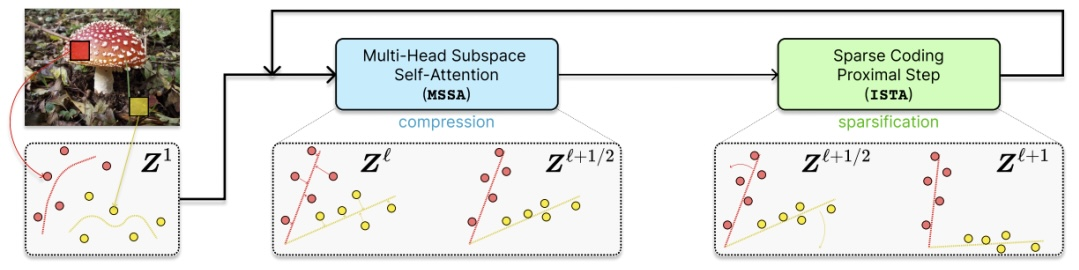
\includegraphics[scale=0.3]{png/think.jpg}
%         % \item 新网络架构CRATE是白盒transformer
%         % \item 表征学习是通过压缩编码和解码实现的:\\
%         % \eee{
%             % \item 他们主要是通过一个注意力机制来将数据先进行了编码,然后用解码器进行解码,这个相比transformer就是只有一个输入和输出,主要谈就他的理解数据的过程.
%         % }
%         \item 关于提示的中间步骤中,他们使用了过程奖励模型(PRM),为每一个推理步骤分配一个参数.\\例如
%         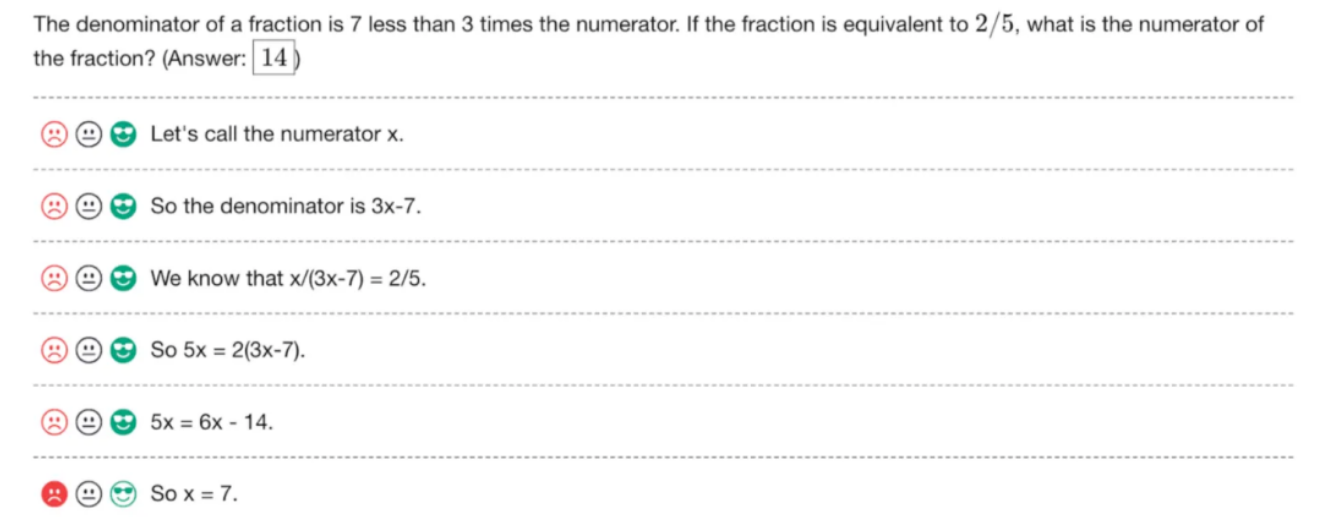
\includegraphics[scale=0.13]{png/process.png}
%     \end{itemize}
% \end{frame}

% \subsection{MLC模型学习基本加减乘法来进行任意数值的计算}
% \begin{frame}
%     \frametitle{模型部署说明}
%     \begin{itemize}
%         \item 模型实现功能:只学习一种规则来对数字完成基本的加减乘以及混合运算.
%         \item 现有模型特点:传统语言模型一般在数字理解能力上比较弱,比如像chatglm类似的语言模型,一般在数字计算上都是通过大量的预训练数据去训练,比如计算3+4=?的时候,现在常见的语言模型都是去回忆以前有没有做过类似的题,而不是理解‘3’,‘+’,‘4’分别指代的意义。因此在数字计算上的能力取决于训练数据,但不管多少训练数据,数字计算是无穷无尽的,模型如果不理解数字就难以拥有具有强大的计算能力。
%         \item 我们的模型希望从数学角度上对数字进行理解。因此通过给定各个数字的运算规则,并给少量运算样例,实现数字的计算。
%         \item 我们模型主要能够实现以下的功能:\\
%             模型自行理解数字,取余以及整除算法,来进行任意数字之间加减乘计算。
%         % \item 模型的一些规律:\\
%         % \eee{
%             % \item 测试的时候和grammar没啥关系。
%             % \item 预测的总长度是有上限的,比如7+3 可以,7+6超过10了,就超出限制了。
%             % \item 根据support中的规则学习到这些多元运算是如何来的,比如二元运算只要学过了,那么任意的数都会了,这个能力就是我们强调的模型对数字的学习能力(*)
%             % \item 示例说明:\\
%             % 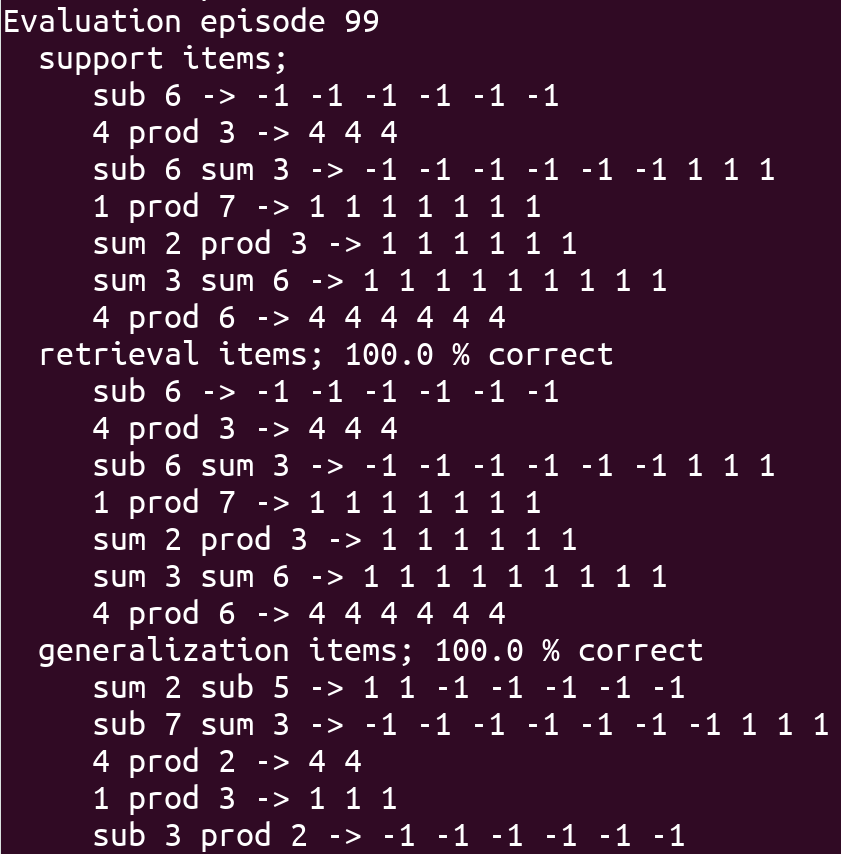
\includegraphics[scale=0.2]{png/result1.png}
%         % }
%     \end{itemize}
% \end{frame}

% % \begin{frame}
% %     \frametitle{模型泛化能力测试结果}
% %     \begin{itemize}
% %         \item 详见代码结果
% %         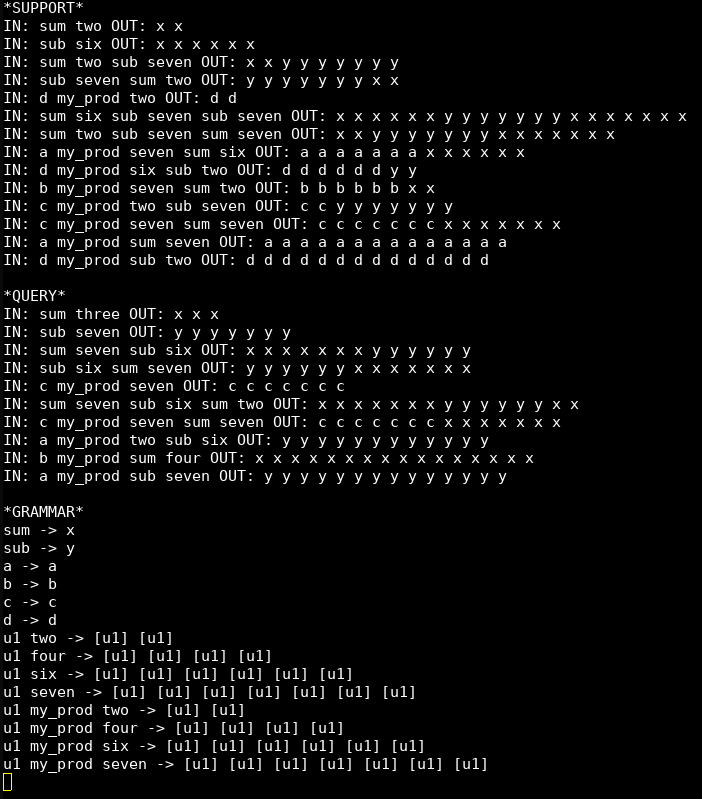
\includegraphics[scale=0.24]{png/test.png}
% %     \end{itemize}
% % \end{frame}

% % \begin{frame}
% %     \frametitle{模型后续改进说明}
% %     \begin{itemize}
% %         \item 目前做的只是10以内的加减乘的数学算法,但可以保证准确性
% %         \item 由于长度的限制,数值变大以后在考虑使用2进制来进行计算.
% %         \item 增加整数的除法.
% %         % \item 当数据变多以后就不确定这样做是否可以继续有效?\\
% %         % \item 还有一些bug需要修改.\\
% %         % 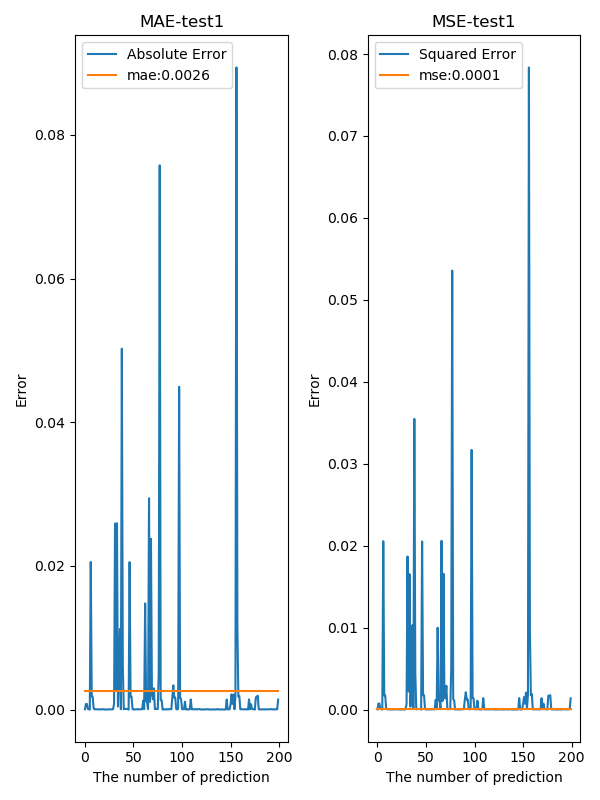
\includegraphics[scale=0.24]{png/test1.png}
% %     \end{itemize}
% % \end{frame}

% % \subsection{序列分类任务测试结果汇总}

% % \begin{frame}
% %     \begin{table}[ht]
% %         \centering
% %         \caption{准确率结果(模型)}        
% %         \large
% %         \label{tab:example}
% %         \begin{tabular}{|c|l|r|c|c| c |}
% %         \hline
% %         模型& lstm & lstm(encoder) & lstm(decoder) & gru\\
% %         \hline        
% %         训练1& {30.99\%} & {31.68\%}& {30.63\%} & {31.58\%} \\
% %         \hline
% %         训练2& {32.85\%} & {31.42\%}& {32.75\%}& {30.06\%}\\
% %         \hline
% %         训练3& {32.09\%} & {28.96\%}& {31.33\%}& {31.87\%}\\
% %         \hline
% %         训练4& {31.63\%} & {32.58\%}& {32.23\%}& {30.18\%}\\
% %         \hline
% %         训练5& {32.36\%} & {30.95\%}& {30.37\%}& {30.76\%}\\
% %         \hline
% %         平均 & {31.98\%} & {31.118\%}& {31.46\%}& {30.89\%}\\
% %         \hline
% %     \end{tabular}
% %         \eee{
% %             % \item 分别在解码器和编码器中引入注意力机制,但是最终效果都不如不加入注意力机制。
% %             % \item 加入注意力机制以后变得更加相比没加之前稳定性有变差.
% %             \item 分别在编码器,解码器引入注意力机制以及lstm的优化模型gru进行对比测试。
% %             \item 从数据结果来看,这个注意力机制对整体的改变影响不大,改进的gru模型由于参数减少使得结果准确度还有所下降。
% %         }
% %         \end{table}
% % \end{frame}

% \begin{frame}
%     \frametitle{加减乘的设计思路}
%     \begin{itemize}
%         \item 首先让模型进行训练学习最基本的乘法,加法表,以及什么是整除,什么是取余,什么是进位。
%         \item 对于任意的两个整数使用模型所理解的加法,进位,进行数字之间的运算。
%         \item 训练数据集示例\\
%         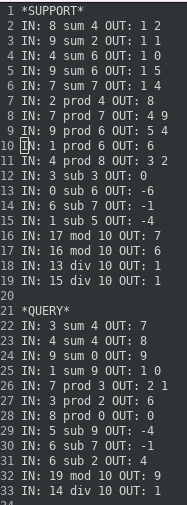
\includegraphics[scale=0.5]{png/example.png}
%     \end{itemize}
% \end{frame}

% \begin{frame}
%     \begin{table}[ht]
%         \centering
%         \caption{MLC模型评估参数}        
%         \large
%         \label{tab:example}
%         \begin{tabular}{|c|l|r|c|c| c |}
%         \hline
%         相关参数 & 数值  \\
%         \hline        
%         最大评估长度 & {20} \\
%         % \hline
%         % 评估中执行的步数数量& {655000} \\
%         \hline
%         模型参数量& {1395344} \\
%         \hline    
%         编码器,解码器层数& {3} \\
%         \hline            
%         多头注意力机制中的头数 & {8}\\
%         \hline
%         dropout & {0.1}\\
%         \hline
%         前馈神经网络的激活函数 & GELU \\
%         \hline
%         \end{tabular}        
%     \end{table}    
% \end{frame}

% \begin{frame}
%     \begin{table}[ht]
%         \centering
%         \caption{准确率结果(模型)}        
%         \large
%         \label{tab:example}
%         \begin{tabular}{|c|l|r|c|c| c |}
%         \hline
%         四则算法种类 & 数据量 & 训练次数 & 准确率  \\
%         \hline        
%         随机5位数加法计算 & {5k} & {100} & {100\%} \\
%         \hline
%         随机6位数加法计算 &  {5k} & {100} & {100\%} \\
%         \hline
%         随机7位数加法计算 & {5k} & {100} & {100\%} \\    
%         \hline
%     \end{tabular}
%         \eee{
%             % \item 分别在解码器和编码器中引入注意力机制,但是最终效果都不如不加入注意力机制。
%             % \item 加入注意力机制以后变得更加相比没加之前稳定性有变差.
%             \item MLC模型在通过训练学习到的数字能力,进行高位数计算,不论数字的位数均可以进行准确的计算得到。
%             % \item 从数据结果来看,这个注意力机制对整体的改变影响不大,改进的gru模型由于参数减少使得结果准确度还有所下降。
%             % \item 100以内的加减计算,使用较少的训练次数就可以达到比较高的准确率了
%             % \item 总的来说,参数量是够的
%         }
%         \end{table}
% \end{frame}

% \begin{frame}
%     \frametitle{训练结果计算图展示(100k,20次)}
%     \begin{itemize}
%         \item 关于100以内数值加减计算(测试结果)\\
%         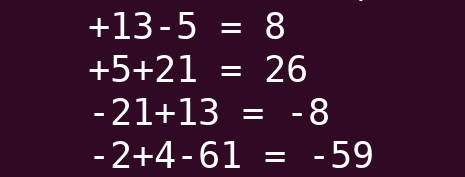
\includegraphics[scale=0.3]{png/number_10_test.png}
%         \item 关于100以内数值加减计算(泛化结果)\\
%         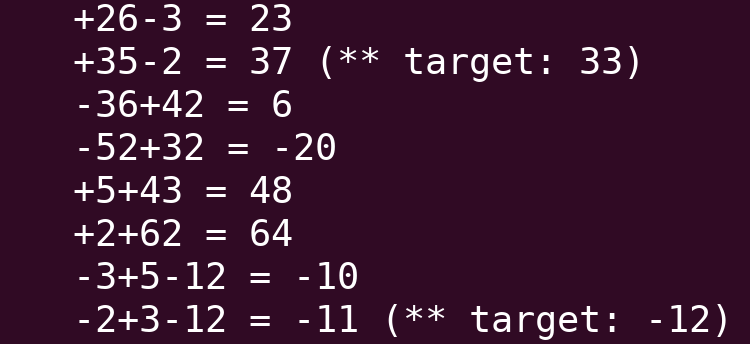
\includegraphics[scale=0.2]{png/number_10_general.png}
%     \end{itemize}    
% \end{frame}

% \begin{frame}
%     \frametitle{训练结果计算图展示(25k,11次)}
%     \begin{itemize}
%         \item 关于100以内数值加减计算(测试结果)\\
%         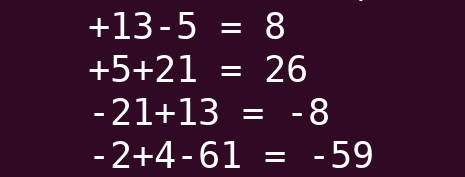
\includegraphics[scale=0.3]{png/number_10_test.png}
%         \item 关于100以内数值加减计算(泛化结果)\\
%         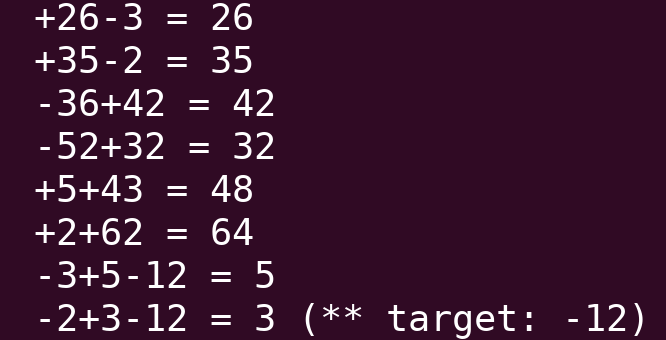
\includegraphics[scale=0.2]{png/number_10_general2.png}
%     \end{itemize}    
% \end{frame}


% \begin{frame}
%     \frametitle{对比差异可视化:多输入多输出结果}
%     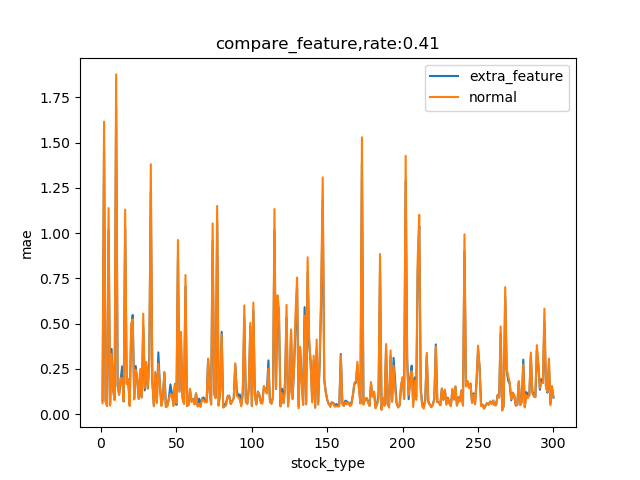
\includegraphics[scale=0.5]{png/much_much.png}
% \end{frame}

% \begin{frame}
%     \frametitle{对比差异可视化:多输入单输出结果}
%     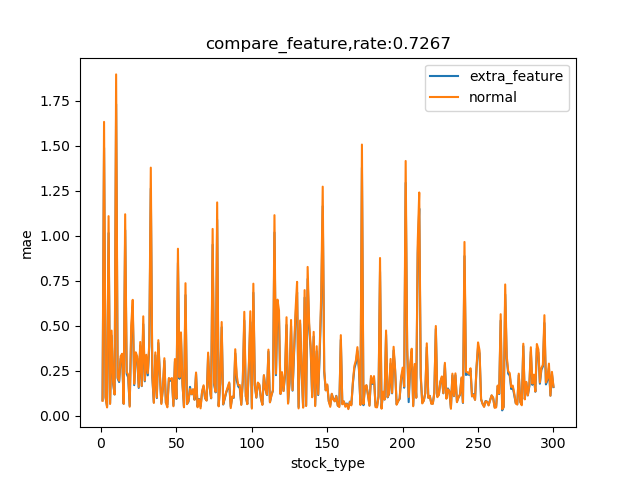
\includegraphics[scale=0.5]{png/much_one.png}
% \end{frame}


% \subsection{模型的修改思路}

% \begin{frame}
% 	\frametitle{}
% 	\begin{itemize}
%         \item 使用频率较高的节点作为基底
%         \eee{
%         \item 将k线图类别中频率最高的前200个作为基底.\\
%         比如将若干个节点组"A,B,D,G,C,...,G,C,G"变成"AB","D","GC",...,"GCG"(个数为25).
%         \item 每次选择25个节点来预测一个节点\\
%         比如根据25个节点:"AB","D","GC",...,"GCG",去预测最后一个节点,比如预测结果是"AB",那么就把"A"作为预测的结果.
%         }
%         \item 
%         关于informer主要做了如下两个修改:
%         \begin{itemize}
%             \item 取消了原本的标准化,数据的标准化以后会导致所有值都在[-1,1]附近不同值之间的特征变得不明显.
%             \item 对于informer的输出部分的线性层和softmax处理器的修改,新增了一层12类别的线性层,并把损失函数从nn.MSELoss()改为nn.CrossEntropyLoss()
%         \end{itemize}        
% 	\end{itemize}
% \end{frame}


    
% \subsection{新的神经网络训练方法——MLC}

% \begin{frame}
%     \frametitle{MLC 是研究人员提出的一种优化程序,旨在通过一系列少样本合成任务来激励系统性}
%     \begin{itemize}
%         \item 探索如何使用元学习技术来帮助模型更好地理解和利用复合性。这可能涉及到训练模型以学习如何组合简单的元素或任务,以构建更复杂的概念或执行更复杂的任务。这个研究领域可能会涉及到深度学习、强化学习、符号推理和其他机器学习方法的结合,以实现更具通用性和适应性的学习系统。其强调如何使用元学习来使模型能够更好地理解和利用任务的复合性,从而提高学习系统的灵活性和性能。
%         \item (数学大模型)DeepMath的效果相当不错,主要是通过高质量数据集的构建,人工标注了几千条现代数学知识问答指令,涵盖了微积分,实分析,复分析,概率论,泛函分析,抽象代数,微分方程,微分几何,拓扑学等多个方向。DeepMath大模型正是基于这个高质量的数据集监督微调llama2语言模型而来。
%     \end{itemize}
% \end{frame}

% \subsection{下一步的计划}
% \begin{frame}
% 	\frametitle{下一步计划及相关问题}	
% 	\begin{itemize}
%         \item 寻找其他相关模型进行比对?
%         % \item 提取模型中的注意力权重,查看模型对于输入信息的处理细节
%         % \eee{
%         %     \item 如何解决经过规范化以后数值比较接近的问题?
%         % }
% 	\end{itemize}
% \end{frame}

% 结束语
\section{}
\begin{frame}
	\frametitle{}
	\begin{center}
		\Huge{谢谢老师和同学们的聆听!}
	\end{center}
\end{frame}

\end{CJK*}
\end{document}
\iffalse 
\begin{frame}
    \frametitle{论文阅读结论}
    \begin{itemize}
        \item 通过动态的组合任务流来引导训练。为了比较人类和机器,我们进行了使用指导学习范式的人类行为实验。在考虑了七种不同的模型后,我们发现,与完全系统但刚性的概率符号模型以及完全灵活但非系统性的神经网络不同,只有MLC实现了人类式概括所需的系统性和灵活性。MLC还在多个系统性概括基准测试中提高了机器学习系统的组合能力。
        我们的结果展示了一种标准神经网络架构,当优化其组合能力时,可以在与人类系统性概括的直接比较中模拟人类系统性概括。
        \item 例如,一旦孩子学会了“跳跃”,他们就能够理解如何“向后跳跃”或“绕锥体跳跃两次”,这是由于他们的组合能力。
        \item 在使用复杂的架构时可以更具系统性。近年来,神经网络取得了显著的进展,并取得了一系列突破,包括在自然语言处理领域
        \item 在本文中,我们提供了证据表明,神经网络可以通过 MLC(一种我们引入的优化过程)实现类似于人类的系统性概括,通过一系列少样本组合任务来鼓励系统性(图1)。我们的MLC实现仅使用常见的神经网络,没有添加符号机制,也没有手工设计的内部表示或归纳偏见。相反,MLC通过高级指导和/或直接人类示例提供了指定所需行为的手段;然后要求神经网络通过元学习来发展正确的学习技能。
        \item 我们展示了MLC如何提高在受欢迎的少样本系统性概括基准测试中的准确性。
        \item 行为结果:
        \eee{
            \item 系统性的泛化通过少样本学习范式进行评估。如图2所示,参与者(n = 25)提供了一套由14个学习指令(输入/输出对)组成的课程,并被要求为10个查询指令生成输出(详细信息请参阅“行为方法:少样本学习任务”部分的方法)。学习指令与潜在的解释语法一致,通过一组组合重写规则从输入中推导出输出(详见“解释语法”部分的方法)。为了表现出色,参与者必须从仅有的几个示例中学习单词的含义,并推广到更复杂的指令。在80.7\%的情况下,参与者能够生成与代数标准完全匹配的输出序列(如图2b(i)中的星号所示)。如果已知长度,两长度输出序列的随机表现为2.8\%,对于更长的序列,随机表现指数减小。值得注意的是,与培训期间看到的较长的输出序列相比,参与者在72.5\%的情况下也能正确推广(如图2b(i)中的最后一条指令所示),这是神经网络经常难以处理的一种泛化类型11。            
            \item 这些响应仍然表现出高度非随机性,具有强烈的归纳偏见。许多错误涉及“一对一”翻译,将每个输入单词精确映射到一个输出符号,就好像所有单词都是原语而不是函数(所有错误中的24.4\%; 如图2b(i)中的1-to-1标记所示)。其他错误涉及应用函数但混淆了其参数,通常以一种表明在保持输入单词顺序与输出符号顺序方面存在“图标串联”偏见的方式(所有涉及函数3的错误中,23.3\%都遵循这种模式;如图2b(i)中的IC标记所示)。这些响应模式可以与更普遍的语言习得中的偏见进行比较;事实上,一对一27和图标串联28,29的形式在自然语言中广泛存在。
            \item 这些归纳偏见通过一个开放性的指令任务进行了更直接的评估,参与者在这个任务中不受学习示例的影响,因此他们的先验偏好更有可能显现出来。不同的人类参与者(n = 29)被要求就七个未知指令的输出以及它们之间的关系进行合理的猜测(对“fep fep”或“fep wif”做出一系列彩色圆圈的响应),而不看任何输入/输出示例以影响他们的回应(有关详细信息,请参阅图3中的完整任务和“方法”部分的“行为方法:开放式任务”)。尽管测试的性质是不受限制的,人们的回应非常有结构,并确认了之前的两种归纳偏见。人们的回应还遵循与相互排斥有关的第三种偏见,该偏见鼓励将独特的含义分配给唯一的词汇27。反映这些偏见的强烈影响,大多数参与者(29人中的17人;58.6\%)的响应都与图3a、b(左侧)中的模式类似,这与所有三种归纳偏见都完全一致。在所有回应中,29名参与者中有18名遵循了一对一(62.1\%),29名参与者中有23名(79.3\%)遵循了图标串联,除两名外,所有参与者都遵循了相互排斥原则,对每个指令产生了唯一的响应(29名参与者中有27名;93.1\%)。
            \item 关于图3的说明:\\
            图3 | 开放式指令任务。a、b,参与者在未看到任何学习示例的情况下对查询(语言字符串)产生了响应(彩色圆圈的序列)。每一列都显示了不同的词汇分配和不同的响应,可以是来自不同参与者(a)或MLC样本(b)。最左侧的模式(a和b中都有)是人和MLC的最常见输出,以一对一(1对1)和从左到右的方式将查询翻译为图标串联(IC)方式。最右侧的模式(a和b中都有)结构不太明显,但仍为每个指令生成唯一的含义(相互排斥(ME))。
            \item 
        }
    \end{itemize}
\end{frame}
\begin{frame}
    \frametitle{第四图}
    \begin{itemize}
        \item 建模结果(特征)
        \eee{
            \item 能够这个过程实在动态变化的情节中进行的
            \item 
        }
        接下来,我们评估了MLC在其产生人类水平的系统性泛化以及在这些具有挑战性的泛化任务上产生类似人类的错误模式的能力。一个成功的模型必须从仅有的几个示例中以系统性的方式学习和使用单词,并倾向于捕捉结构化的输入/输出关系的假设。MLC的目标是引导神经网络到参数数值,以便在面对未知任务时支持正是这些种类的泛化并克服以前对系统性的限制。重要的是,这种方法旨在模拟成年人的组合技能,而不是成年人获得这些技能的过程,这是在一般讨论中进一步考虑的问题。MLC的源代码和预训练模型可在线上获得(代码提供)
        \item 如图4所示,详细内容请参阅“方法”部分的“架构和优化器”部分,MLC使用标准的变换器架构26进行基于内存的元学习。MLC优化变换器以响应新的指令(查询输入),给定一组输入/输出对(学习示例;也称为支持示例21),所有这些都被连接在一起并一起传递作为输入。这相当于元学习,因为优化是在动态变化的情节中进行的(每个情节都有新的学习和查询示例),而不是在静态数据集上进行的;具体而言,每个情节构成了一个不同的seq2seq任务30,31,通过随机生成的潜在语法来解释输入作为输出(请参阅“MLC和MLC变体的元训练程序”部分)。为了成功,变换器必须找到能够从学习的单词中提取含义并将它们组合以回答查询的参数值,依赖于元学习,同时也依赖于变换器架构的创新,这些创新在Fodor和Pylyshyn的论点中没有预见到1(例如,可变长度输入、参数共享和自我关注)。在测试情节中,模型的权重被冻结,不提供任务特定的参数32。最后,鉴于模拟人类响应(包括错误)是最终目标,我们随机地将每个查询与代数输出序列(通过情节的语法生成)或启发式输出序列(通过一对一翻译或错误应用规则进行采样)配对,采样比例大致与经验观察到的比例相同(请参阅“MLC和MLC变体的元训练程序”部分)。
        \item MLC能够优化高度系统化行为的模型。最系统的运行产生了一个变换器,当在与人们相同的少样本指令学习任务中选择最佳响应时,该变换器表现得完全系统化(100\%的精确匹配准确度)(图2;详细信息请参阅“方法”的“评估程序”部分以及模型变异性在10次运行中的补充信息1),而且还能够推断出未参与元学习的新规则(补充信息1)。对这次运行的非正式分析进一步显示,MLC还能够表现出更微妙和受偏见驱使的行为;从模型输出的分布中进行采样时(图2b),变换器以接近人类表现(80.7\%)的平均率(82.4\%)生成系统化的输出,并以接近人类水平(72.5\%)的速度适当处理较长的输出序列(77.8\%)。此外,与人们一样,LC变换器会产生反映一对一翻译(56.3\%的错误;人类为24.4\%)和图标级串联(13.8\%涉及函数3的错误;人类为23.3\%)的错误。MLC还可以预测哪些指令对人们来说更容易或更困难(皮尔逊相关系数为0.788,P = 0.031,双尾置换检验,n = 10项;详见扩展数据图1中的项目级性能)。在正式表格1(少样本学习)中,我们通过给定模型预测33所有人类响应(图2b (i))的对数似然来比较模型。在本段的其余部分,当我们说一个模型胜过另一个模型时,它们之间的自然对数点差大于等于8。MLC变换器(表1;MLC)在预测人类行为方面优于更为严格系统化的模型。这包括一个概率符号模型,假设人们推断出黄金语法但偶尔会出现任意的失误(符号(oracle);方法部分提供了所有符号和基本seq2seq模型的详细信息),以及一个在与MLC相同的训练情节上优化的变换器,尽管输出响应是严格代数的(而不是基于偏见)(MLC(仅代数);方法部分提供了所有MLC变体的详细信息)。MLC还优于一个基本的seq2seq变换器,该变换器适应图2中的模式而没有进行元学习,以及一个MLC模型,其优化目标是复制而不是系统性的概括(MLC(仅复制);在培训过程中,查询示例总是与学习示例之一匹配)。MLC变换器在假设人们推断出黄金语法但根据人类归纳偏见进行偶然失误的概率符号模型方面表现得与其相媲美(符号(oracle/biases))。事实上,MLC同样被优化为(隐式)推断出系统化规则并以相同的基于偏见的模式做出回应,因此这两个模型表现出相似是很自然的。性能最佳的MLC(联合)在少样本学习任务和开放式人类响应中都经过了联合优化,如下一段所述。
        \item 尽管人类的少样本学习行为可以由MLC或概率符号模型很好地表征,但对更为开放的行为的测试强调了MLC的相对优势。相同的变换器体系结构经过了优化,以在开放式参与者行为中填充输出,然后一次性为七个指令填写输出(图3;详细信息请参阅“方法”的“评估程序”部分)。MLC变换器在65.0\%的样本中完全如模型人类参与者回应(图3b(左)),完美地体现了三个关键的归纳偏见。进一步的非正式分析还揭示了MLC捕获了更微妙的响应模式,只部分使用归纳偏见(图3b(右))。在所有模型样本中,有66.0\%遵循一对一(人类为62.1\%),85.0\%遵循图标级串联(人类为79.3\%),绝大多数(99.0\%)选择了每个唯一命令的唯一响应(人类为93.1\%)。模型预测还通过五折交叉验证33进行了评估:MLC和其他模型分别针对23或24名参与者的响应进行了优化(具体取决于交叉验证的拆分),然后为留出的参与者预测响应。通过对数似然评分,并在表1(开放式)中进行总结(在五次交叉验证拆分上求和,平均在三次运行中)。在本段的其余部分,当我们说一个模型胜过另一个模型时,差异大于等于57个自然对数点。MLC优于所有其他选择,包括在先前实验中描述的高度代数的MLC模型(仅代数)和一个概率符号模型,该模型使用三个归纳偏见生成响应,但与MLC不同,它不能优化人类行为中的其他模式(表1;符号(oracle/biases))。重要的是,单个变换器可以针对少样本学习和开放式指令任务进行优化(MLC(联合));事实上,这是跨实验预测人类行为的最强大模型(扩展数据图5和补充信息1中显示了额外的分析)。
    \end{itemize}
\end{frame}
\begin{frame}
    \frametitle{机器学习基准测试}
    \begin{itemize}
        \item 机器学习基准测试
        除了预测人类行为之外,MLC可以在系统化泛化的机器学习基准测试中实现低于1\%的错误率。请注意,这里用于优化的示例是由基准测试设计者通过代数规则生成的,因此没有直接模仿人类行为数据。我们尝试了两个流行的基准测试,SCAN和COGS,重点关注它们的系统化词汇泛化任务,探究对新单词和单词组合的处理(而不是新的句子结构)。MLC仍然只使用标准的变压器组件,但为了处理更长的序列,根据“机器学习基准测试”方法部分的描述,添加了处理学习示例的模块化。
        SCAN涉及将指令(如“走两次”)翻译成一系列动作(“走走”)。在“添加跳跃”分组中,训练集只有一个关于如何“跳跃”(映射到“跳跃”)的示例,测试集探讨了这个动词的组成用法(例如,“跳来跳去右转两次,走三次”),与我们的人类学习任务类似(“zup”类似于图2中的“跳跃”)。
        COGS涉及将句子(例如,“一个气球被Emma画了”)翻译成表达其含义的逻辑形式(balloon(x 1 )∨ draw.theme(x 3 ,x 1 )∨ draw.agent(x 3 ,Emma))。COGS评估了21种不同类型的系统化泛化,其中大多数检查了名词和动词的一次性学习。为了鼓励少样本推理和意义组合,我们依赖表层词类排列,这是元学习的一个简单变种,它使用最少的结构性知识,详见“机器学习基准测试”方法部分。这些排列通过单词的表面类型改变而不扩展基准测试的词汇,以逼近更具自然性的新单词的不断引入(图1)。
        基准测试错误率总结在表2中。在SCAN上,MLC解决了三个系统化泛化分组,错误率低至0.22\%或更低(准确率高达99.78\%或更高),包括前面提到的“添加跳跃”分组以及“围绕右转”和“对面右转”,检查已知单词的新组合。在COGS上,MLC在18种词汇泛化类型中实现了0.87\%的错误率。没有进行元学习的基本seq2seq在基准测试中的错误率至少是MLC的七倍,尽管使用了相同的变压器架构。但是,表面层次的排列对于MLC来说不足以解决基准测试中的结构泛化任务。MLC无法处理更长的输出序列(SCAN长度分组)以及更复杂的句子结构(COGS中的三种类型),错误率为100\%。这些任务需要处理“生产力”(参见参考文献1第33页),这在很大程度上不同于系统性。但是,在我们的少样本指令学习任务中,MLC确实处理了新的句子结构(对于具有比学习过程中看到的更长的输入和输出序列的查询,正确率为77.8\%,如图2所示),这表明正确的元训练程序可以促进生产力,这是我们将来要解决的问题。 
    \end{itemize}
\end{frame}
\begin{frame}
    \frametitle{讨论}
讨论
35多年前,当Fodor和Pylyshyn提出了神经网络中系统性的问题1时,今天的模型19及其语言技能可能是难以想象的。作为对Fodor和Pylyshyn的预见能力的肯定,系统性辩论一直存在。系统性仍然挑战着模型11-18并激发了新的框架34-41。在补充信息3中报告的初步实验表明,即使对于最新的大型语言模型(如GPT-4)来说,系统性仍然是一个挑战,或者至少是一个未解之谜。
为了解决这一辩论,并了解神经网络是否能够捕捉类似于人类的组合技能,我们必须将人类和机器进行并排比较,就像在本文和其他最近的工作7,42,43中一样。在我们的实验中,我们发现人类最常见的响应方式在Fodor和Pylyshyn1讨论的方式上是代数和系统性的。然而,人们还依赖归纳偏见,有时支持代数解决方案,有时偏离代数解决方案;事实上,人们不是纯粹的代数机器3,6,7。我们展示了MLC如何使标准的神经网络经过优化以实现其组合技能,以模仿或超越人类的系统性泛化在并排比较中。MLC的系统性远远强于以标准方式训练的神经网络,并且比纯粹的符号模型表现出更复杂的行为。MLC还允许神经网络处理其他现有挑战,包括使用孤立基元进行系统化使用11,16以及使用相互排斥来推断含义44。我们使用MLC进行行为建模与其他逆向工程人类归纳偏见的方法相关。贝叶斯方法使建模者能够评估不同的表现形式和参数设置,以捕捉通过模型先验45指定的人类行为,这些先验也可以通过分层贝叶斯建模46与行为数据进行调整,尽管结果设置可能会受到限制。MLC展示了如何使用元学习来逆向工程归纳偏见(参见参考文献47,了解正式的关系),尽管需要使用更大的表现能力的神经网络。我们的研究增加了一篇关于使用元学习来理解人类或类似人类行为的文献,以前已经进行了综述48,涉及元学习。在我们的实验中,只有MLC密切复制了人类的行为,包括系统性和偏见,MLC ( joint)模型在这两种蓝图之间的权衡方面最好。
此外,MLC通过元学习获得其能力,系统性泛化和人类偏见不是神经网络架构的固有属性,而是从数据中诱导出来的。
尽管取得了成功,MLC并不能解决Fodor和Pylyshyn1中提出的所有挑战。MLC不能自动处理未经训练的泛化形式或在元学习分布之外的概念,降低了完全新颖结构的范围,它可以正确处理(比较在补充信息1中报告的学习新规则的令人鼓舞的结果与它在SCAN和COGS生产力分组上的失败)。此外,MLC无法概括对其进行优化的归纳偏见的微妙差异,因为我们通过补充信息2中的额外行为和模型实验进一步探讨。用机器学习的语言来说,我们认为元学习策略在泛化使新的情节在与训练情节相关分布时成功,在与情节中呈现的学习示例不相关时特定测试项是不成功的。当前的架构也缺乏发出新符号的机制2,尽管通过额外的指针机制55可以发出通过学习
\end{frame}

\fi